\documentclass[10pt,a4paper]{article}
\usepackage[utf8]{inputenc}
\usepackage[a4paper, total={6in, 8in}]{geometry}
\usepackage{graphicx}
\usepackage{adjustbox}
\usepackage{subcaption}
\usepackage{amsmath}
\usepackage{booktabs}
\usepackage{float}
\begin{document}
\begin{titlepage}
\begin{center}
\newcommand{\HRule}{\rule{\linewidth}{0.5mm}}
% Upper part of the page. The '~' is needed because \\
% only works if a paragraph has started.

\includegraphics[width=0.15\textwidth]{./SwanseaLogo}~\\[1cm]

\textsc{\LARGE University of Swansea}\\[1.5cm]

\textsc{\Large Project Report 2}\\[0.5cm]

% Title
\HRule \\[0.4cm]
{ \huge \bfseries Project Report 2\\ April $22^{nd}$ 2015 \\[0.4cm] }

\HRule \\[1.5cm]

% Author and supervisor
\noindent
\begin{minipage}{0.4\textwidth}
\begin{flushleft} \large
\emph{Author:}\\
Robert \textsc{James}
\end{flushleft}
\end{minipage}%
\begin{minipage}{0.4\textwidth}
\begin{flushright} \large
\emph{Supervisor:} \\
Professor Biagio \textsc{Lucini}
\end{flushright}
\end{minipage}

\vfill

% Bottom of the page

\end{center}

\clearpage

\end{titlepage}


\section{Progress}



\subsection{Results}
For the Wang Landau Algorithm, I need two target parameters the target energy and target width.
To verify that the Wang Landau sampling algorithm was working correctly, I used the theoretical result for $\beta_c = \ln(1+\sqrt(q))$ as the $\beta$ value in the regular metropolis.
Taking the average energy result from the metropolis algorithm over 100 different runs I then used this value as the target energy.
I then averaged the results for various grid sizes to get a target energy that would be compatible with all of the grid sizes I would test in the next stage.
Taking the target width to be the length of the lattice which is the same as in the Guagnelli paper\cite{guagnelli}.
The average results are given in the table below.

\begin{table}[h]
\centering
\begin{adjustbox}{width=1\textwidth}
\begin{tabular}{cccccccccc}
\hline
\multicolumn{9}{|c|}{Q2} & \multicolumn{1}{c|}{Average} \\ \hline
\multicolumn{1}{|c|}{8} & \multicolumn{1}{c|}{10} & \multicolumn{1}{c|}{12} & \multicolumn{1}{c|}{14} & \multicolumn{1}{c|}{16} & \multicolumn{1}{c|}{18} & \multicolumn{1}{c|}{20} & \multicolumn{1}{c|}{22} & \multicolumn{1}{c|}{24} & \multicolumn{1}{c|}{-} \\ \hline
\multicolumn{1}{|c|}{-1.746055} & \multicolumn{1}{c|}{-1.73125} & \multicolumn{1}{c|}{-1.70554} & \multicolumn{1}{c|}{-1.709935} & \multicolumn{1}{c|}{-1.729} & \multicolumn{1}{c|}{-1.699675} & \multicolumn{1}{c|}{-1.7202} & \multicolumn{1}{c|}{-1.697715} & \multicolumn{1}{c|}{-1.71876} & \multicolumn{1}{c|}{-1.71757} \\ \hline
\multicolumn{1}{l}{} & \multicolumn{1}{l}{} & \multicolumn{1}{l}{} & \multicolumn{1}{l}{} & \multicolumn{1}{l}{} & \multicolumn{1}{l}{} & \multicolumn{1}{l}{} & \multicolumn{1}{l}{} & \multicolumn{1}{l}{} & \multicolumn{1}{l}{} \\ \hline
\multicolumn{9}{|c|}{Q3} & \multicolumn{1}{c|}{Average} \\ \hline
\multicolumn{1}{|c|}{8} & \multicolumn{1}{c|}{10} & \multicolumn{1}{c|}{12} & \multicolumn{1}{c|}{14} & \multicolumn{1}{c|}{16} & \multicolumn{1}{c|}{18} & \multicolumn{1}{c|}{20} & \multicolumn{1}{c|}{22} & \multicolumn{1}{c|}{24} & \multicolumn{1}{c|}{-} \\ \hline
\multicolumn{1}{|c|}{-1.655655} & \multicolumn{1}{c|}{-1.635225} & \multicolumn{1}{c|}{-1.59797} & \multicolumn{1}{c|}{-1.59217} & \multicolumn{1}{c|}{-1.62166} & \multicolumn{1}{c|}{-1.567135} & \multicolumn{1}{c|}{-1.6117} & \multicolumn{1}{c|}{-1.563485} & \multicolumn{1}{c|}{-1.62098} & \multicolumn{1}{c|}{-1.607331111} \\ \hline
\multicolumn{1}{l}{} & \multicolumn{1}{l}{} & \multicolumn{1}{l}{} & \multicolumn{1}{l}{} & \multicolumn{1}{l}{} & \multicolumn{1}{l}{} & \multicolumn{1}{l}{} & \multicolumn{1}{l}{} & \multicolumn{1}{l}{} & \multicolumn{1}{l}{} \\ \hline
\multicolumn{9}{|c|}{Q4} & \multicolumn{1}{c|}{Average} \\ \hline
\multicolumn{1}{|c|}{8} & \multicolumn{1}{c|}{10} & \multicolumn{1}{c|}{12} & \multicolumn{1}{c|}{14} & \multicolumn{1}{c|}{16} & \multicolumn{1}{c|}{18} & \multicolumn{1}{c|}{20} & \multicolumn{1}{c|}{22} & \multicolumn{1}{c|}{24} & \multicolumn{1}{c|}{-} \\ \hline
\multicolumn{1}{|c|}{-1.60852} & \multicolumn{1}{c|}{-1.594505} & \multicolumn{1}{c|}{-1.541865} & \multicolumn{1}{c|}{-1.513065} & \multicolumn{1}{c|}{-1.573255} & \multicolumn{1}{c|}{-1.494005} & \multicolumn{1}{c|}{-1.55854} & \multicolumn{1}{c|}{-1.498545} & \multicolumn{1}{c|}{-1.56628} & \multicolumn{1}{c|}{-1.549842222} \\ \hline
\multicolumn{1}{l}{} & \multicolumn{1}{l}{} & \multicolumn{1}{l}{} & \multicolumn{1}{l}{} & \multicolumn{1}{l}{} & \multicolumn{1}{l}{} & \multicolumn{1}{l}{} & \multicolumn{1}{l}{} & \multicolumn{1}{l}{} & \multicolumn{1}{l}{} \\ \hline
\multicolumn{9}{|c|}{Q8} & \multicolumn{1}{c|}{Average} \\ \hline
\multicolumn{1}{|c|}{8} & \multicolumn{1}{c|}{10} & \multicolumn{1}{c|}{12} & \multicolumn{1}{c|}{14} & \multicolumn{1}{c|}{16} & \multicolumn{1}{c|}{18} & \multicolumn{1}{c|}{20} & \multicolumn{1}{c|}{22} & \multicolumn{1}{c|}{24} & \multicolumn{1}{c|}{-} \\ \hline
\multicolumn{1}{|c|}{-1.61393} & \multicolumn{1}{c|}{-1.513115} & \multicolumn{1}{c|}{-1.454555} & \multicolumn{1}{c|}{-1.49718} & \multicolumn{1}{c|}{-1.53578} & \multicolumn{1}{c|}{-1.459115} & \multicolumn{1}{c|}{-1.54886} & \multicolumn{1}{c|}{-1.37051} & \multicolumn{1}{c|}{-1.540035} & \multicolumn{1}{c|}{-1.503675556} \\ \hline
\multicolumn{1}{l}{} & \multicolumn{1}{l}{} & \multicolumn{1}{l}{} & \multicolumn{1}{l}{} & \multicolumn{1}{l}{} & \multicolumn{1}{l}{} & \multicolumn{1}{l}{} & \multicolumn{1}{l}{} & \multicolumn{1}{l}{} & \multicolumn{1}{l}{} \\ \hline
\multicolumn{9}{|c|}{Q10} & \multicolumn{1}{c|}{Average} \\ \hline
\multicolumn{1}{|c|}{8} & \multicolumn{1}{c|}{10} & \multicolumn{1}{c|}{12} & \multicolumn{1}{c|}{14} & \multicolumn{1}{c|}{16} & \multicolumn{1}{c|}{18} & \multicolumn{1}{c|}{20} & \multicolumn{1}{c|}{22} & \multicolumn{1}{c|}{24} & \multicolumn{1}{c|}{-} \\ \hline
\multicolumn{1}{|c|}{-1.63928} & \multicolumn{1}{c|}{-1.561295} & \multicolumn{1}{c|}{-1.53851} & \multicolumn{1}{c|}{-1.45837} & \multicolumn{1}{c|}{-1.633735} & \multicolumn{1}{c|}{-1.31854} & \multicolumn{1}{c|}{-1.508195} & \multicolumn{1}{c|}{-1.3654} & \multicolumn{1}{c|}{-1.5185} & \multicolumn{1}{c|}{-1.504647222} \\ \hline
\end{tabular}
\end{adjustbox}
\caption{Every value is averaged for 100 different random seeds. Calculated using a random position approach}
\end{table}

As stated above, to verify that the Wang Landau model that I had implemented in the code was returning accurate results I needed to confirm that the $a_n$ returned for the energy at $\beta$ were compatible.
In the thermodynamic limit, the aforementioned theoretical results would be as described below.

\begin{table}[h]
\centering
\begin{tabular}{|c|c|}
\hline
Q & $\beta_c$ \\ \hline
2 & 0.881373587 \\ \hline
3 & 1.005052539 \\ \hline
4 & 1.098612289 \\ \hline
8 & 1.342454046 \\ \hline
10 & 1.426062439 \\ \hline
\end{tabular}
\caption{Theoretical $\beta_c$ in the Thermodynamic Limit}
\end{table}

To verify that the results I obtained from the Wang Landau algorithm are compatible with the $\beta$ values I ran the program $30$ times on various different lattice sizes.
Taking those averages and plotting against the inverse volume would lead to a straight line plot that should intercept the y-axis at $\beta_c$.

A summarized table of results for $Q=2$ is below, the other results can be found at the end of the report.

\begin{table}[h]
\centering
\begin{adjustbox}{width=1\textwidth}
\begin{tabular}{ccccccccc}
\hline
\multicolumn{9}{|c|}{Grid Size} \\ \hline
\multicolumn{1}{|c|}{8} & \multicolumn{1}{c|}{10} & \multicolumn{1}{c|}{12} & \multicolumn{1}{c|}{14} & \multicolumn{1}{c|}{16} & \multicolumn{1}{c|}{18} & \multicolumn{1}{c|}{20} & \multicolumn{1}{c|}{22} & \multicolumn{1}{c|}{32} \\ \hline
\multicolumn{1}{|c|}{-} & \multicolumn{1}{c|}{-} & \multicolumn{1}{c|}{-} & \multicolumn{1}{c|}{-} & \multicolumn{1}{c|}{-} & \multicolumn{1}{c|}{-} & \multicolumn{1}{c|}{-} & \multicolumn{1}{c|}{-} & \multicolumn{1}{c|}{-} \\ \hline
\multicolumn{1}{|c|}{1.019009633} & \multicolumn{1}{c|}{0.8149062} & \multicolumn{1}{c|}{0.9067844667} & \multicolumn{1}{c|}{0.9228866667} & \multicolumn{1}{c|}{0.9028289667} & \multicolumn{1}{c|}{0.9047848} & \multicolumn{1}{c|}{0.8716884333} & \multicolumn{1}{c|}{0.8674836} & \multicolumn{1}{c|}{0.8770940333} \\ \hline
\multicolumn{1}{l}{} & \multicolumn{1}{l}{} & \multicolumn{1}{l}{} & \multicolumn{1}{l}{} & \multicolumn{1}{l}{} & \multicolumn{1}{l}{} & \multicolumn{1}{l}{} & \multicolumn{1}{l}{} & \multicolumn{1}{l}{} \\
\multicolumn{1}{l}{} & \multicolumn{1}{l}{} & \multicolumn{1}{l}{} & \multicolumn{1}{l}{} & \multicolumn{1}{l}{} & \multicolumn{1}{l}{} & \multicolumn{1}{l}{} & \multicolumn{1}{l}{} & \multicolumn{1}{l}{}
\end{tabular}
\end{adjustbox}
\caption{The row of '-' represents the 30 non averaged results. The final result is shown}
\end{table}

Plotting these results against the inverse volume and linearly fitting the data against $f(x) = a * x + b$.

\begin{figure}[H]
\centering
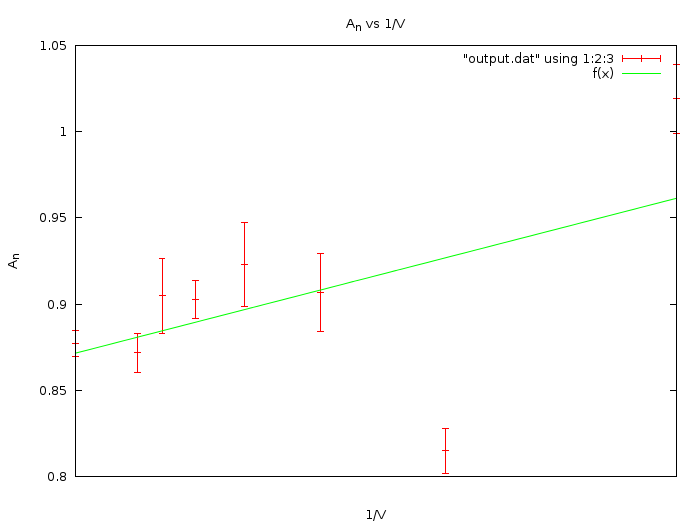
\includegraphics[width=0.75\textwidth]{q2variousgrid.png}
\caption{$a_n$ values from various grid sizes at critical energy}
\end{figure}

The final value for the intercept after fitting against the datafile.
\begin{equation}
\begin{split}
f(x) = a x + b \\
a = 6.12898 \pm 4.229 \textrm{ (69\%)}\\
b = 0.865616 \pm 0.03173     \textrm{ (3.666\%)}
\end{split}
\end{equation}

As you can see in the section above, the fitted y intercept was $0.865616 \pm 0.03173$ the theoretical result was $0.881373587$ meaning the returned result was correct within error.
Below are the graphs and the final fitted values with errors.

\begin{figure}
\centering
\begin{subfigure}[b]{0.45\textwidth}
    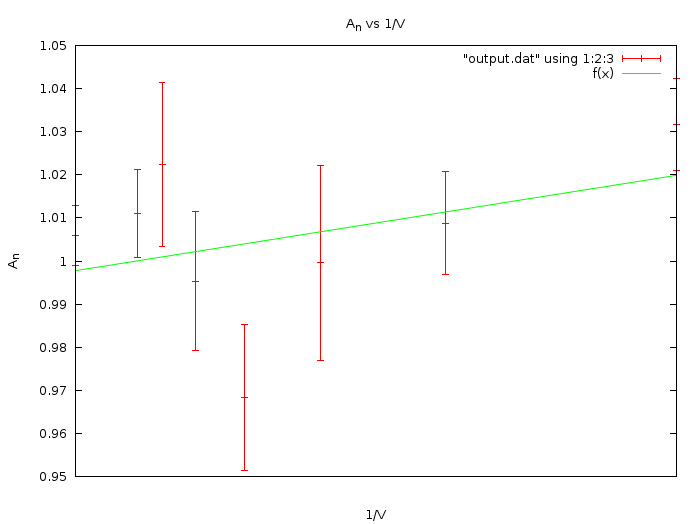
\includegraphics[width=\textwidth]{q3variousgrid.png}
    \caption{Q3 $a_n = 0.996294 \pm 0.01123$}
\end{subfigure}
\begin{subfigure}[b]{0.45\textwidth}
    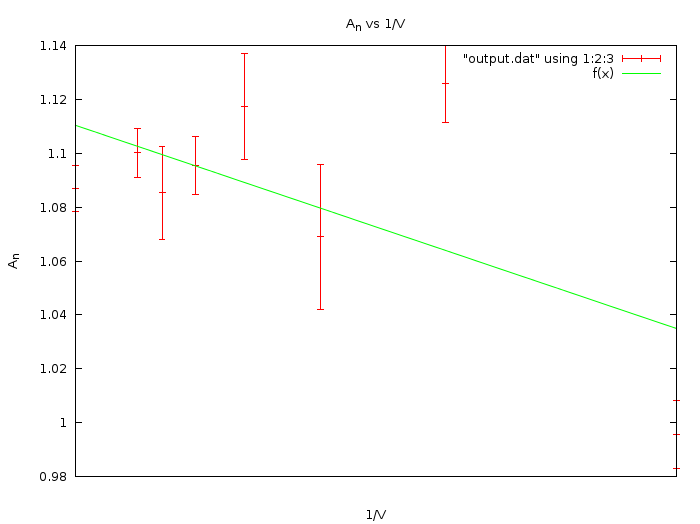
\includegraphics[width=\textwidth]{q4variousgrid.png}
    \caption{Q4 $a_n = 1.11538 \pm 0.02026$}
\end{subfigure}

\begin{subfigure}[b]{0.45\textwidth}
    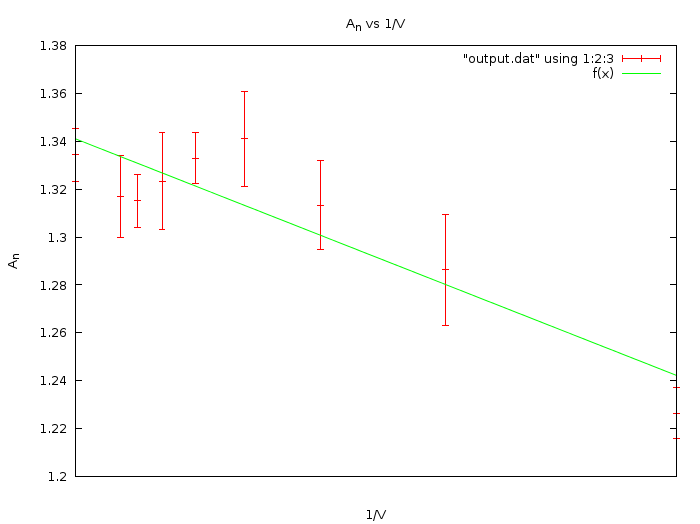
\includegraphics[width=\textwidth]{q8variousgrid.png}
    \caption{Q8 $a_n = 1.34759 \pm 0.008933$}
\end{subfigure}
\begin{subfigure}[b]{0.45\textwidth}
    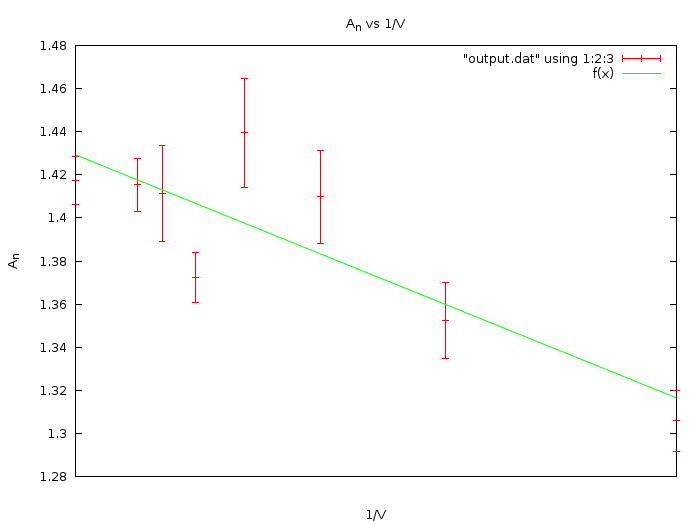
\includegraphics[width=\textwidth]{q10variousgrid.png}
    \caption{Q10 $a_n = 1.43679 \pm 0.0152$}
\end{subfigure}
\end{figure}

After showing that the results fitted the theoretical within errors, I moved onto the next stage of the project.
To calculate the partition function of the lattice without an interface we need to first calculate the density of states.
The density of states can be expanded using a Taylor Series expansion when the energy is in the neighbourhood of the target energy.

\begin{equation}
\log{g(E)} = a_{n}+c(E_0)
\end{equation}

The next step is to generate $a_n$ for various energies to allow us to calculate the local linear approximation of the density of states.

\begin{figure}
  \centering
  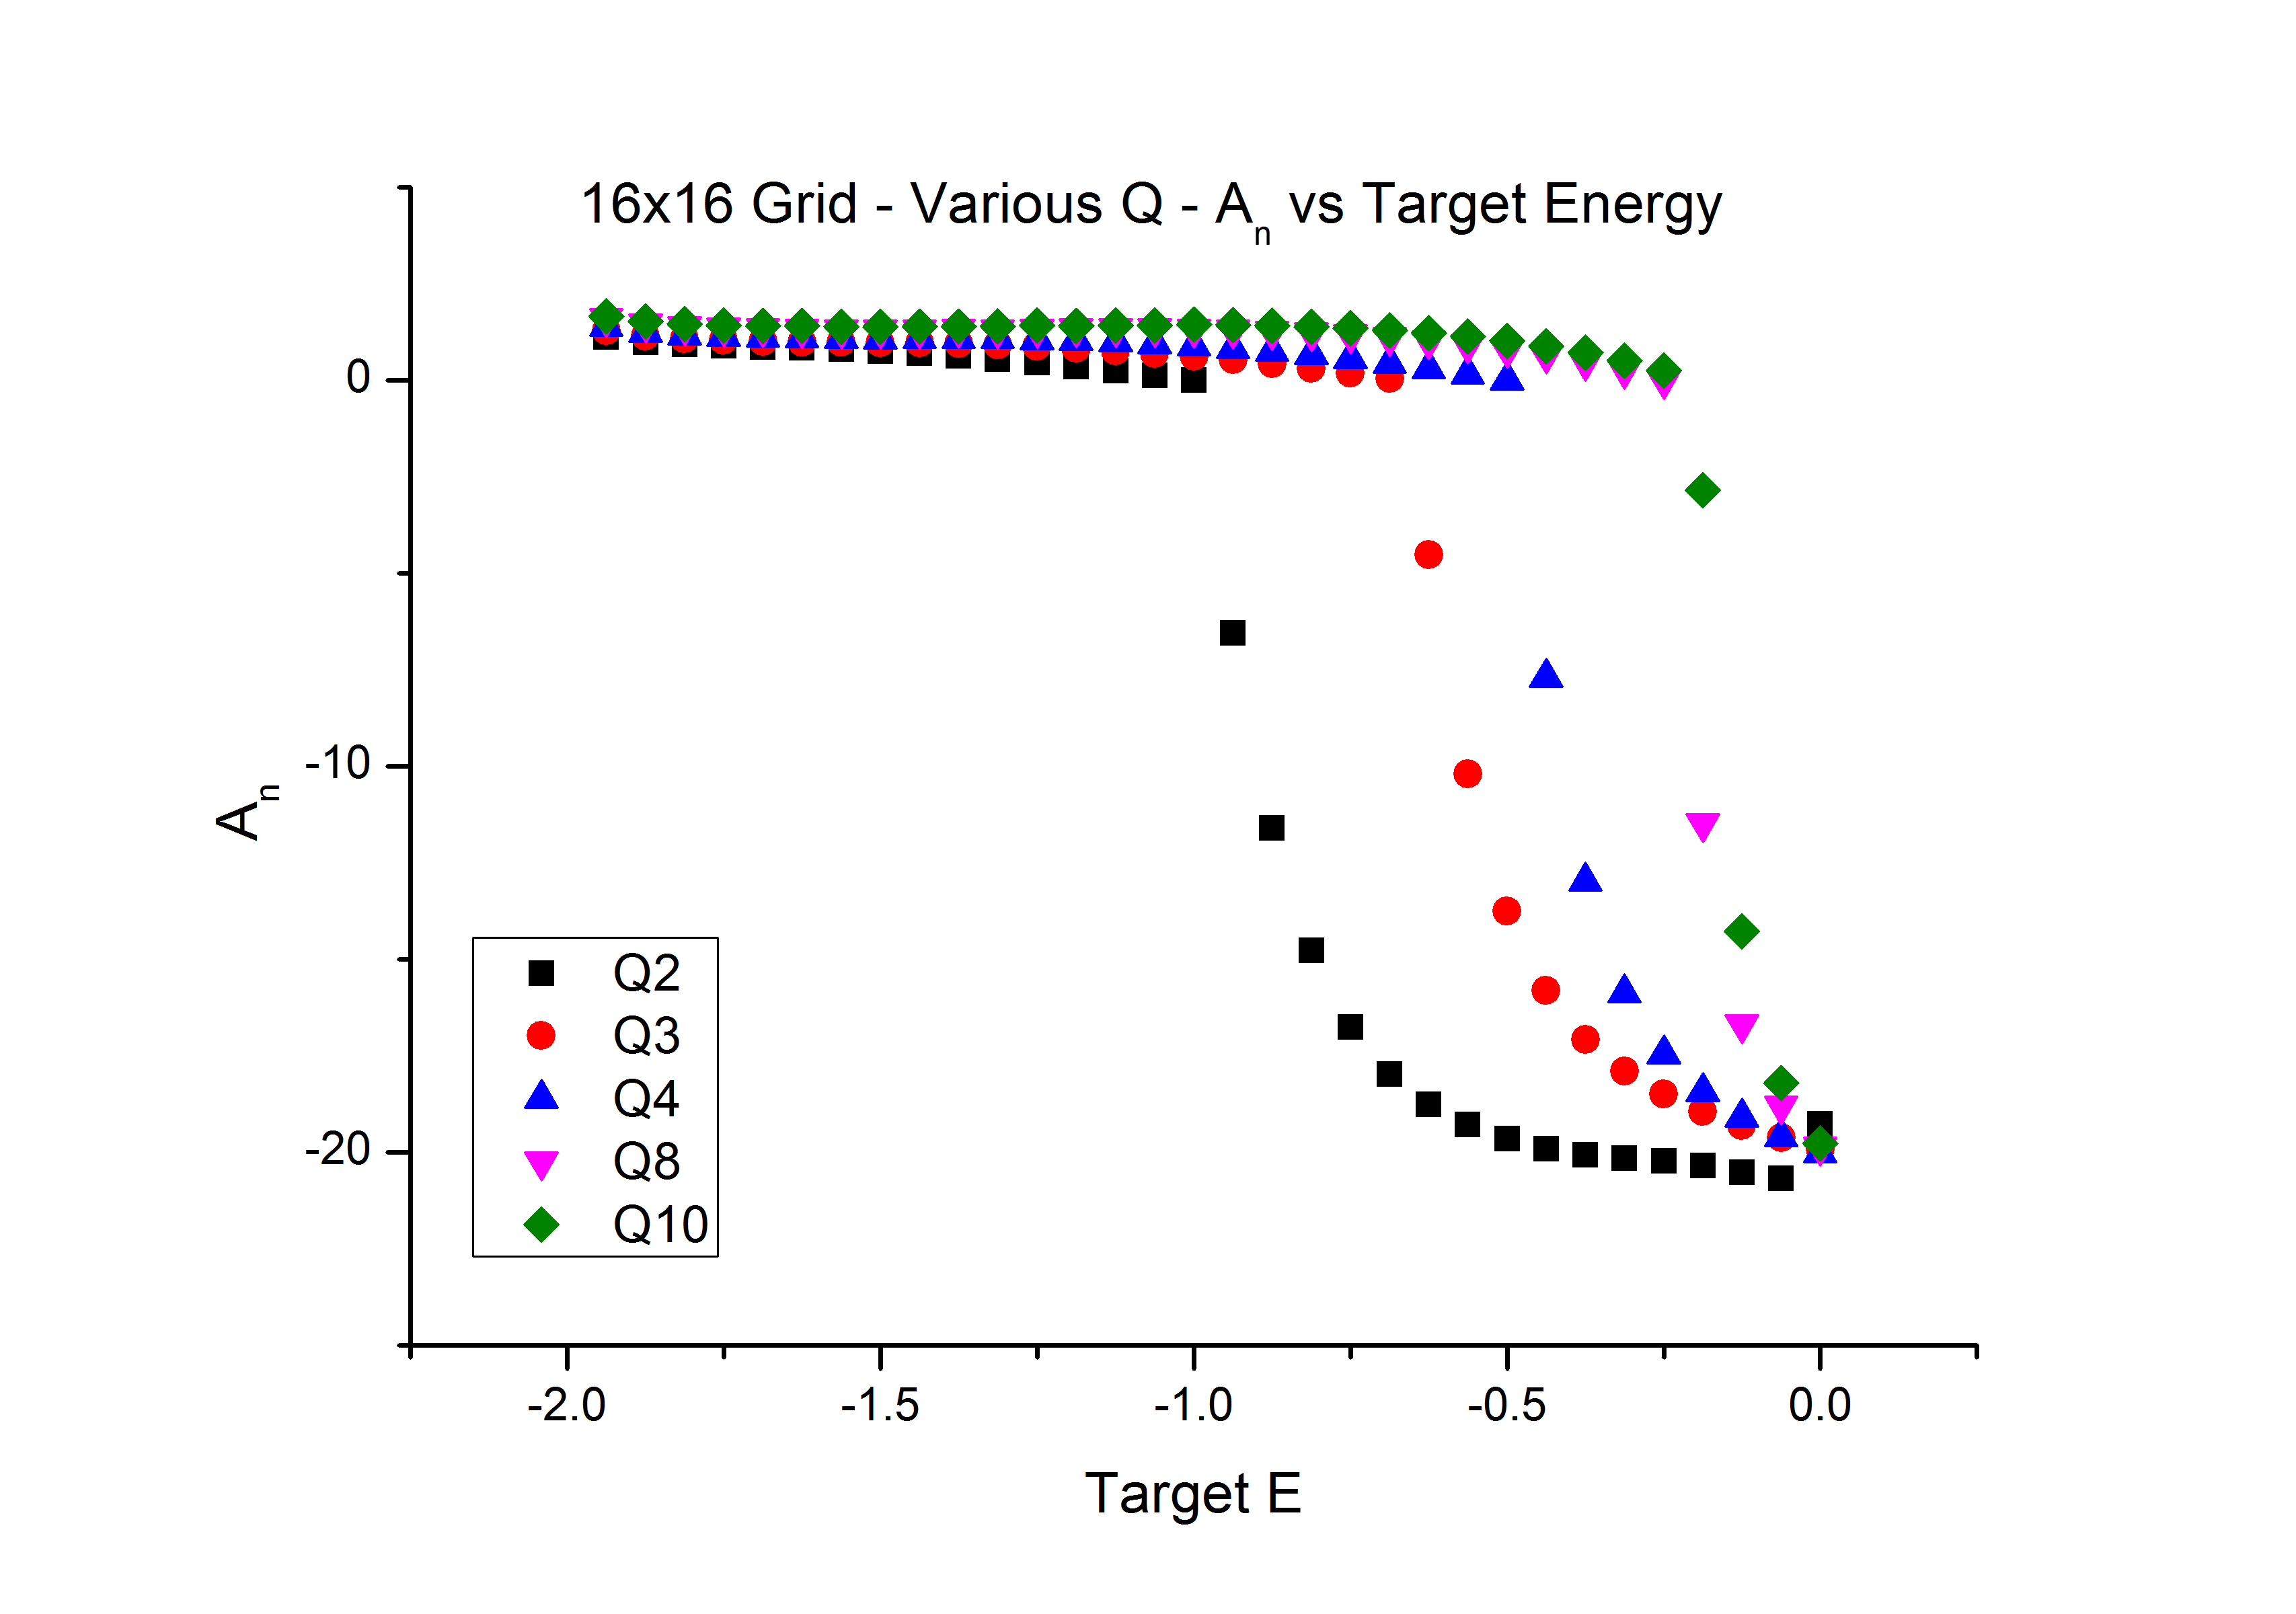
\includegraphics[width=\textwidth]{variousq16x16-full.png}
  \caption{Plot of $a_n$ vs Target Energy for Various Q on a 16x16 lattice}
\end{figure}

As you can see, changing the Target Energy of the Wang Landau inside the range of $-2 V$ to $0$.
Leads to some \textit{interesting} results. $\beta$ is inversely proportional to the temperature.
While negative $T$ is possible in some specific ultracold atom experiments it doesn't seem physical in this particular case.
To this end, from the earlier experiments I discovered correlation to $q$ in the maximum energy that was reached.
\begin{equation}
    E_{Max} = -2 \frac{1}{q}
\end{equation}

While this behaviour is unexpected, the earlier results seem to suggest that the particular algorithm implementation leads to this result.
As Q increases the number of possible combinations that would lead to the maximum energy increases.
Despite the fact that this is likely an implementation issue, the end result is that the data just needs to be examined inside the range relavent to it's specific q.

Following from that, after removing the extra data you find that the plot becomes significantly more useable and revealing.
The type of phase transition changes when $q>4$.
Looking at the graph below there is a clear change in the behaviour for $q>4$.
For $q>4$ you can see regions of stability around the point of transition.

\begin{figure}[h]
    \centering
    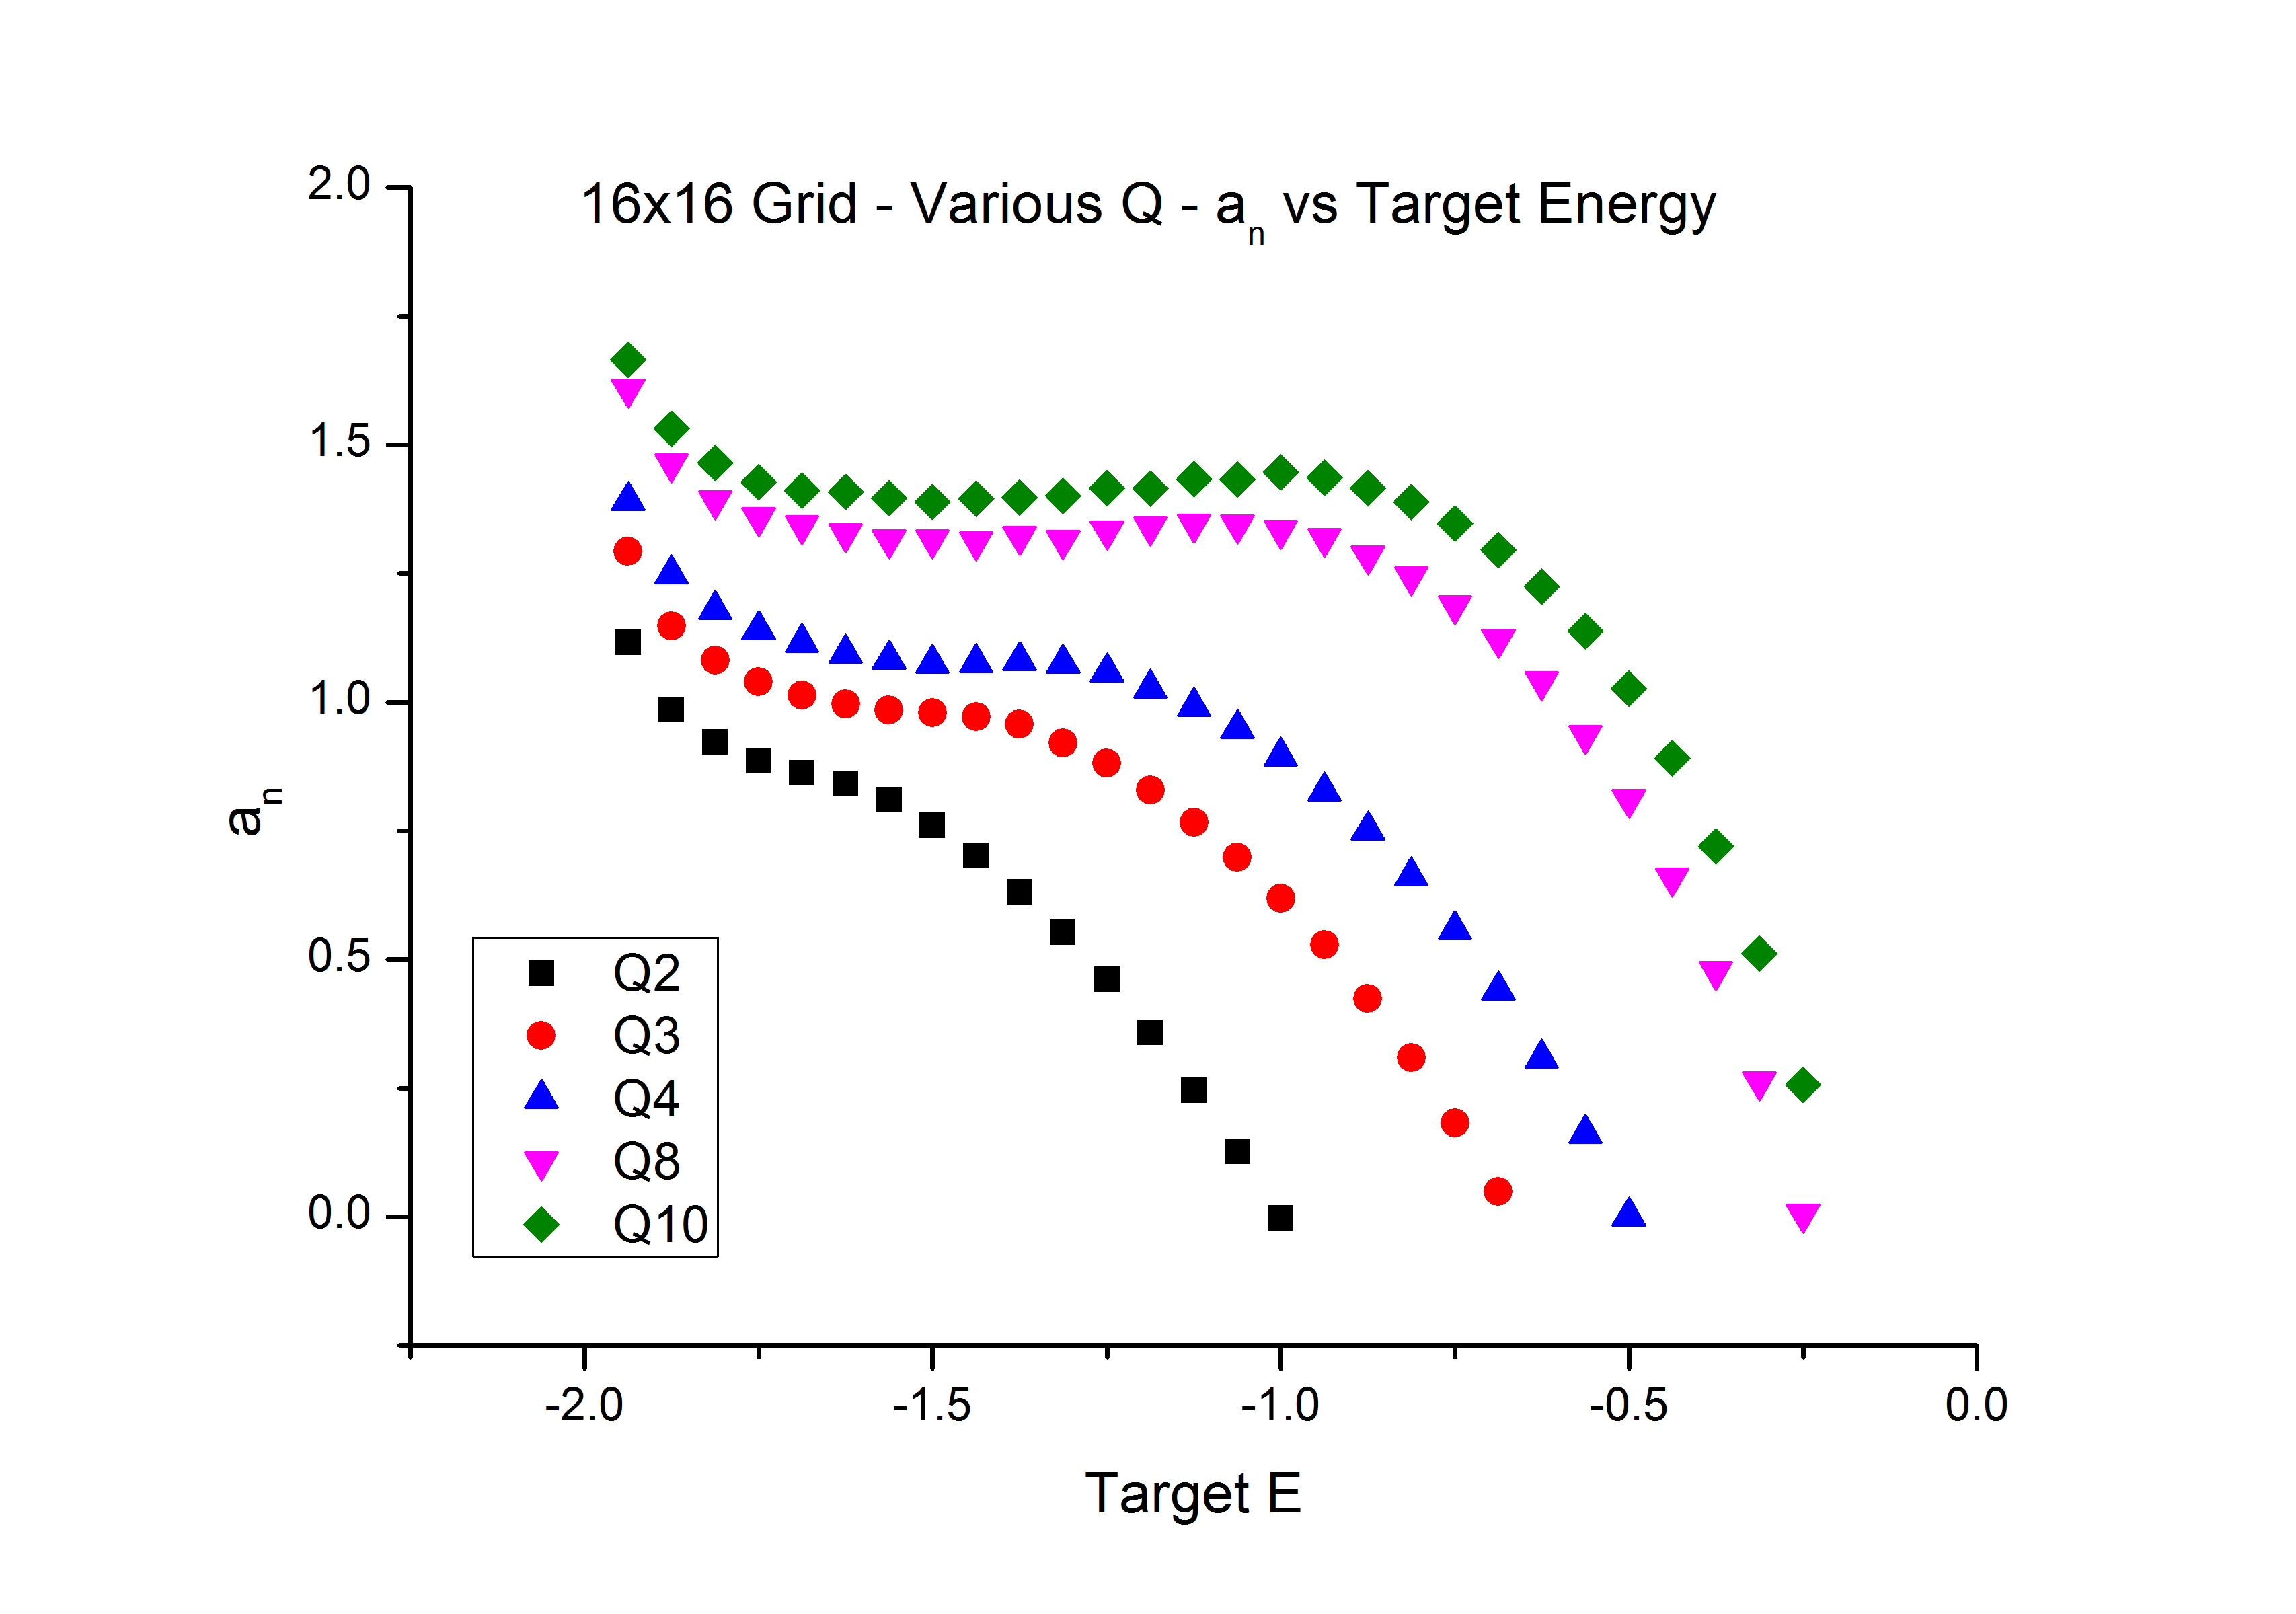
\includegraphics[width=0.75\textwidth]{variousq16x16.png}
    \caption{Restricted Plot of $a_n$ vs Target Energy for Various Q on a 16x16 lattice}
\end{figure}

Focusing on $q=10$ now, you can see behaviour very similar to that in the Guagnelli paper which suggests that the behaviour is correct.
Below is a plot that looks at the $a_n$ around the critical point of $q=10$ $\beta_c = 1.426062439$.
\begin{figure}[h!]
    \centering
    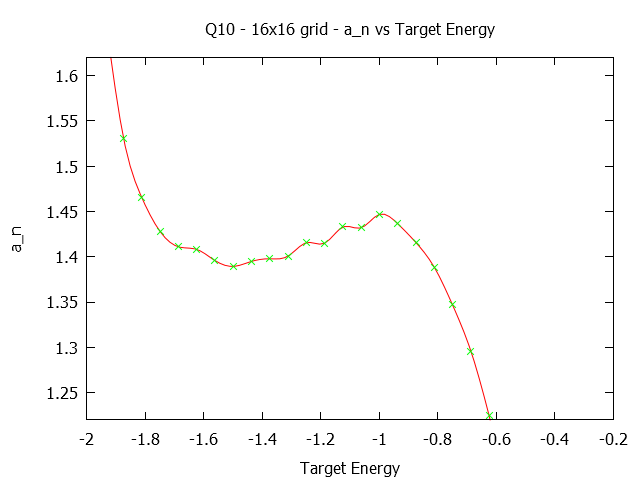
\includegraphics[width=0.75\textwidth]{q1016x16.png}
    \caption{$q=10$ for comparison against Guagnelli}
\end{figure}

Using the linear approximation and the fact that $E_{i}+\delta = E_{i+1}-\delta$. You can construct an equation for the DoS (Density of States).
In Mathematica I imported the data to a workbook and calculated the linear components of the Density of States.
\begin{equation}
\text{Con}(\text{n$\_$})\text{:=}\text{delta} \left(2 \sum _{i=1}^n \text{Q2data}[[i]]+\text{Q2data}[[n]]+\text{Q2data}[[1]]\right)+\text{C0}
\end{equation}
The above equation allows you to calculate each of the constants from the $a_n$ data at the midpoints.
For a Grid Size of 8 the parameters for Q2,Q3,Q4,Q8 and Q10 are given below.
\begin{table}[h]
\begin{tabular}{|c|c|c|c|c|c|}
\hline
Q & 2 & 3 & 4 & 8 & 10 \\ \hline
Constants & $2.07489+C_0$ & $2.80549+C_0$ & $3.38889+C_0$ & $4.77754+C_0$ & $5.2132+C_0$ \\ \hline
\end{tabular}
\end{table}

\section{Future}
Next thing to do is calculate $C_0$ this require numerically calculating the below integral.
\begin{equation}
    C_0 = \ln{\frac{Z(0)}{\int r(E) dE}} = \ln{\frac{2L^2}{\int r(E) dE}}
\end{equation}
After that I need to implement a different version of the code thus far that for a specific column in the lattice applies a different delta function.
\begin{equation}
    H = \sum_{i,j!=(k,*)}\delta_{i,j} + \sum_{i,j=(k,*)}\delta_{i,(j+k)modq}
\end{equation}
Where $ 0 <= k < L$ this will enforce a boundary/interface onto the lattice.
Doing the same analysis on this new lattice to produce a partition function will lead to the $\mathcal{Z}^*$ of that lattice.
The next step will be to calculate the Free Energy of the interface.
This will involve the ratio of the standard partition function and that of the modified lattice.
\begin{equation}
F_{I}(L)=-\log(\frac{\mathcal{Z}^{*}(L)}{\mathcal{Z(L)}}) + \log(L)
\end{equation}


\bibliographystyle{plain}
\bibliography{References}

\end{document}
